\documentclass[11pt,a4paper]{article}
\usepackage[top=40px, left=60px, right=60px]{geometry}
\usepackage[T1]{fontenc}
\usepackage[normalem]{ulem}
\usepackage{verbatim}
\usepackage[utf8]{inputenc}
\usepackage[francais]{babel}
\usepackage{graphicx}
\usepackage{placeins}
\usepackage{listings}
\usepackage{color}

\definecolor{mauve}{rgb}{0.58,0,0.82}
\lstset{ %
	basicstyle=\footnotesize\ttfamily,
	frame=single
}

\title{Factorisation d'entiers}
\author{Stéphane Horte \& Gabriel Lewertowski}

\begin{document}
\maketitle

\tableofcontents

\begin{abstract}
Nous présentons trois algorithmes de factorisation d'entiers : les algorithmes \textit{$\rho$} et \textit{$(p-1)$} proposés par J.M Pollard en 1974 dans \cite{pollard_rho} ainsi que l'algorithme \textit{ECM} (Elliptic Curve Method) décrit par H. W. Lenstra, Jr dans \cite{lenstra}. Nous testons ensuite nos implémentations sur des grands nombres choisis aléatoirement, et nous comparons avec les résultats obtenus par GMP-ECM.
\end{abstract}

\section{ECM, hier et aujourd'hui}
La méthode ECM a été proposée par H. W. Lenstra en 1985 \cite{lenstra}, et peu d'améliorations ont été apportées depuis. Alors qu'à ses débuts, l'algorithme permet de trouver des facteurs premiers de 30 chiffres au maximum, R. Brent prédit qu'ECM permettra à l'avenir de trouver des facteurs premiers de 50 chiffres. En effet, dix ans plus tard en 1995, P. Montgomery trouve un facteur de 47 chiffres de $5^{256} +1$. L'actuel record est un facteur de 83 chiffres, trouvé en septembre 2013 par R. Propper en factorisant $7^{337}+1$ \cite{records_ecm}. \\

P. Montgomery et R. Propper se sont intéressés à ces nombres dans le cadre du Projet Cunningham, lancé en 1925 et visant à factoriser des entiers de la forme $b^n \pm 1$ avec $b \in \{2, 3, 5, 6, 7, 10, 11, 12\}$ et $n$ grand. ECM fait partie, avec le crible algébrique et le crible quadratique à polynômes multiples, des trois seuls algorithmes utilisés récemment pour factoriser ces nombres. \\

Aujourd'hui, l'algorithme ECM est le meilleur algorithme de factorisation connu parmi ceux pour lesquels la complexité dépend de la taille du facteur trouvé et pas de la taille de l'entier à factoriser : on ne considère donc pas le crible quadratique et le crible algébrique, dont les complexités respectives en fonction de l'entier $n$ à factoriser valent $O\left(e^{\sqrt{\log n\log\log n}}\right)$ et $O\left(e^{(\frac{64}{9}\log n)^{\frac{1}{3}}(\log\log n)^{\frac{2}{3}}}\right)$. \\

L'implémentation la plus rapide de l'algorithme ECM est GMP-ECM, un programme développé en C par des chercheurs de l'INRIA, permettant de factoriser un entier avec les méthodes $p-1$, $p+1$ et ECM.

\subsection{Fonctionnement de GMP-ECM}
Le programme prend en paramètre la borne $B1$ de l'étape 1 et un ou plusieurs entiers à factoriser depuis   l'entrée standard. Par exemple, pour factoriser un entier avec $B1 = 10^6$ :


\begin{figure}[!h]
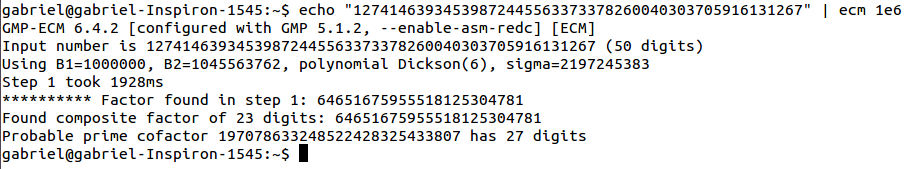
\includegraphics[scale=0.5]{images/gmp-ecm1.png}
\end{figure}

Par défaut, la méthode utilisée est ECM. On peut utiliser $(p-1)$ avec l'option -pm1 : 

\begin{lstlisting}[language=bash]
	echo "12652209139612535291" | ecm -pm1 1e6
\end{lstlisting}

L'utilisateur peut également spécifier une valeur de $B_2$ pour la phase 2. Par exemple, pour utiliser $B_1=10^6$ et $B_2=10^9$ : 

\begin{lstlisting}[language=bash]
	echo "12652209139612535291" | ecm 1e6 1e9
\end{lstlisting}

Si aucune valeur de $B_2$ n'est spécifiée, GMP-ECM détermine automatiquement la valeur de $B_2$ optimale en fonction de la taille de l'entier à factoriser.
\medskip

\begin{tabular}{|c|c|c|c|}
  \hline
  Nb de chiffres de $N$ & $B_1$ optimal & $B_2$ optimal & Nb de courbes à utiliser \\
  \hline
  20 & 11e3 & 1.9e6 	& 74  \\
  25 & 5e4 & 1.3e7 & 214 \\
  30 & 25e4 & 1.3e8 & 430 \\
  35 & 1e6 & 1.0e9 & 904 \\
  40 & 3e6 & 5.7e9 & 2350 \\
  45 & 11e6 & 3.5e10 & 4480 \\
  50 & 43e6 & 2.4e11 & 7553 \\
  55 & 11e7 & 7.8e11 & 17769 \\
  60 & 26e7 & 3.2e12 & 42017 \\
  65 & 85e7 & 1.6e13 & 69408 \\
  \hline
\end{tabular}

\subsection{Détails de l'implémentation}
L'algorithme ECM tel que présenté en 1985 par Lenstra sélectionnait aléatoirement la courbe elliptique sur laquelle travailler. P. Montgomery a proposé en 1987 dans \cite{montgomery} une amélioration pour travailler avec une famille infinie de courbes dont l'ordre est divisible par 12, ce qui augmente la probabilité de succès puisque l'algorithme ECM réussit si l'ordre du groupe n'a que des petits facteurs. C'est cette famille de courbes qu'utilise GMP-ECM, avec la paramétrisation 
\[
by^2z = x^3 + ax^2z + xz^2
\]
qui permet une addition et une multiplication rapides. \\

Lors de la phase 2, GMP-ECM a recours à l'extension de Brent-Suyama qui, au lieu de calculer $b^s$ pour $s$ un nombre premier dans l'intervalle $[B_1, B_2]$, calcule $b^{(6k)^e - 1}$ avec $k$ un entier et $e$ un petit entier pair. Cette extension utilise la remarque suivante : tout nombre premier strictement supérieur à 3 est de la forme $6k \pm 1$. Pour plus de détails sur l'extension de Brent-Suyama et l'évaluation multipoints, voir \cite{zimmerman}.

\begin{thebibliography}{9}
\bibitem{pollard_rho}
J. M. Pollard, \emph{A Monte Carlo method for factorization}, BIT, 1975, pp.331-334

\bibitem{lenstra}
H. W. Lenstra, Jr, \emph{Factoring integers with elliptic curves}, Annals of Mathematics, 1987, pp.649-673

\bibitem{montgomery}
P. Montgomery, \emph{Speeding the Pollard and Elliptic curve methods of factorization}, American Mathematical Society, jan. 1987, pp. 243-264

\bibitem{zimmerman}
P. Zimmerman, \emph{GMP-ECM: yet another implementation of the Elliptic Curve Method}, conférence.

\bibitem{records_ecm}
http://www.loria.fr/~zimmerma/records/top50.html


\end{thebibliography}

\end{document}
